\documentclass[%
 reprint,
 amsmath,amssymb,
 aps,
]{revtex4-2}

\usepackage{hyperref}
\usepackage{xcolor}
\usepackage{braket}
\usepackage{subcaption}
\usepackage{pdfcomment}
\usepackage{todonotes}
\usepackage[nolist,nohyperlinks]{acronym}
\usepackage{amsmath, amsthm, amssymb, amsbsy, mathtools, mathalpha}

\usepackage{graphicx}% Include figure files
\usepackage{dcolumn}% Align table columns on decimal point
\usepackage{bm}% bold math
\usepackage{hyperref}% add hypertext capabilities
\usepackage{color, units}
\usepackage[normalem]{ulem}

\usepackage{xspace}
% \usepackage{subfigure}
\usepackage{comment}
\usepackage{xcolor}
%\usepackage[mathlines]{lineno}% Enable numbering of text and display math
%\linenumbers\relax % Commence numbering lines



\DeclareMathOperator{\argmax}{argmax} % no space, limits on side in displays
\DeclareMathOperator{\argmin}{argmin} % no space, limits on side in displays


\graphicspath{{figures/}}



\newcommand{\avi}[1]{\textcolor{orange}{[Avi: #1]}}
\newcommand{\RM}[1]{\textcolor{red}{[RM: #1]}}
\newcommand{\kl}[1]{\textcolor{violet}{Kate : #1}}
\newcommand{\KJ}[1]{\textcolor{teal}{KJ : #1}}


\newcommand{\citeme}{\textcolor{red}{[CITEME]}}
\newcommand{\vect}[1]{\boldsymbol{#1}}
\renewcommand{\d}{{\bf d}}
\newcommand{\bnu}{\mbox{\boldmath $\nu$}}
\newcommand{\btheta}{\mbox{\boldmath $\theta$}}
\newcommand{\bdelta}{\mbox{\boldmath $\delta$}}
\newcommand{\balpha}{\mbox{\boldmath $\alpha$}}
\renewcommand{\S}{{\bf S}}
\newcommand{\A}{{\bf A}}
\newcommand{\Y}{{\bf Y}}
\newcommand{\Z}{{\bf Z}}

\newcommand{\Sn}{\ensuremath{S_n^{\mathrm{GP}}}}
\newcommand{\tmes}{\ensuremath{{\mkern-2mu\times\mkern-2mu}}}
\newcommand{\ex}[1]{\ensuremath{\tmes10^{\text{-}#1}}}

\newcommand{\hyperopt}{\texttt{HyperOpt}}



\begin{document}

\preprint{APS/123-QED}


\title{
Fast power spectral density estimation \\
for correlated multivariate detector noise \\
using variational inference
}% Force line breaks with \\

\author{Jianan Liu}
\author{Nelson Christensen}
\author{Kamiel Janssens}%
\author{Jeung Eun Lee}
\author{Patricio Maturana-Russel}
\author{Renate Meyer}
\author{Avi Vajpeyi}

 \email{Second.Author@institution.edu}
\affiliation{University of  Auckland}%
\collaboration{NZ Gravity}%\noaffiliation

\date{\today}% It is always \today, today,
             %  but any date may be explicitly specified

\begin{abstract}
 This paper presents a novel spectral density estimation method that applies to very long multivariate time series such as those encountered when analyzing data from a network of detectors such as the Einstein Telescope or LISA. The method introduces a blocked Whittle likelihood approximation for stationary time series and makes use of the Cholesky decomposition of the inverse spectral density matrix to obtain a positive definite spectral density estimator. A prior is placed on the spline coefficients of each Cholesky factor and a stochastic gradient variational Bayes approach is used to compute the posterior distribution. We illustrate the method using x seconds of simulated correlated ET noise.\ldots
 %We illustrate this technique for ET noise characterisation and simultaneous extraction of a binary merger signal.  For computational feasibility we approximate the posterior distribution the variational Bayesian method, minimizing the KL divergence with the variational distribution. As the result, we can estimate the spectral density quite accurately and quickly. 
\end{abstract}

%\keywords{Suggested keywords}%Use showkeys class option if keyword
                              %display desired
\maketitle


% Acronyms
\begin{acronym}
    \acro{GW}[GW]{gravitational-wave}
    \acro{GWs}[GWs]{gravitational-waves}
    \acro{ET}[ET]{Einstein Telescope}
    \acro{LISA}[LISA]{Laser Interferometer Space Antenna}
    \acro{CE}[CE]{Cosmic Explorer}
    \acro{PE}[PE]{parameter estimation}
    \acro{PSD}[PSD]{Power Spectral Density}
    \acro{DFT}[DFT]{Discrete Fourier Transform}
    \acro{SNR}[SNR]{Signal-to-Noise Ratio}
    \acro{BBH}[BBH]{binary black hole}
    \acro{VI}[VI]{variational inference}
    \acro{KL}[KL]{Kullback-Leibler}
    \acro{MCMC}[MCMC]{Markov chain Monte Carlo}
    \acro{LVK}[LVK]{LIGO--VIRGO--KAGRA}
\end{acronym}


\section{Introduction}

% Introduce detectors
The next-generation gravitational wave detectors, e.g. \ac{ET}~\cite{Punturo_2010}, \ac{CE}~\cite{CE_horizon_study}, and \ac{LISA}~\cite{LISA_science_case}, will usher in a transformative era of gravitational wave astronomy. 
The increased sensitivity to gravitational waves will lead to a much higher gravitational wave detection rate, improving our understanding of cosmic phenomena, ranging from the dynamics of black hole mergers to the nature of the early universe~\cite{ET_science_case, Maggiore_2020_ET_science_case, Branchesi_2023_ET_science_case, CE_horizon_study, LISA_science_case}.


% introduce challenge of correlated noise 
Although next-generation detectors will be more sensitive than current detectors, they face novel challenges such as the characterisation of correlated multivariate noise~\cite{ET_design_report,LISA_design_report}.
\ac{ET} and \ac{LISA} consist of co-located interferometers, leading to correlated noise between their data streams~\cite{Janssens2023}. For \ac{ET}, some of these correlated noise sources can be attributed to seismic, Newtonian, and magnetic noise~\cite{Ball_lightning_strokes, Janssens_newtonian_seismic, Janssens_magnetic_noise}. 
In the case of \ac{LISA}, the correlated noise sources could be from temperature variations~\cite{lisa_temp_noise} and mico-thrusters~\cite{lisa_thrusters_noise}. 

% talk about issues of ignoring correlated noise
The implications of neglecting correlated noise in \ac{PE} analyses of gravitational waves can lead to biased parameter estimates and erroneous conclusions regarding astrophysical phenomena~\cite{Thrane_correlations_SGWB, Christensen_2019_SGWB, Cireddu:2023:arXiv, boileau2022figures}. For example, consider the impact of noise correlation in \ac{PE} for the stochastic \ac{GW} background~\cite{boileau2022figures} or transient signals from events such as binary black hole mergers~\cite{Cireddu:2023:arXiv}. Although \citet{Cireddu:2023:arXiv} and \citet{JanssensKamiel2023Ffps} have introduced the likelihood of a correlated network of GW detectors and a formula for the power and cross-power spectral densities, a flexible Bayesian approach to estimating the matrix-valued spectral density function is still to be developed. Such an approach needs to be nonparametric, i.e., robust w.r.t.\ deviations from certain parametric shapes such as power laws in order to be able to capture all potential small- and large-scale noise characteristics.
Furthermore, the approach needs to be computationally efficient when applied to very long time series of GW observations. \citet{MeierAlexander2020Bnao} and \citet{LiuYixuan2024Ancl} have developed a nonparametric Bayesian approach to multivariate spectral density estimation based on the Whittle likelihood and a positive semidefinite matrix-Gamma process prior on the spectral density matrices and used an adaptive MCMC algorithm to sample from the posterior. While theoretically attractive with proven consistency properties and contraction rates, MCMC methods are notoriously slow and require a large amount of computation time, thus are only applicable to small- to medium-sized time series. 



% past work in tackling correlated noise.
% Past work.....
\todo{Talk about past work trying to tackle correlated noise.}

% what will this work do? 
In this paper, we demonstrate a stochastic gradient \ac{VI} approach to estimate the multivariate \ac{PSD} for correlated \ac{ET} noise that has been developed by \cite{Hu2023}. 
\ac{VI} operates by refining the parameters of a surrogate posterior distribution, minimising the \ac{KL} divergence between this surrogate and the actual posterior distribution \cite{Jordan1999,Wainwright2008,Blei2017}. As the surrogate is tuned closer to the true posterior, the sampling efficiency increases, making inference trivial. 
VI transforms complex integration and posterior sampling tasks into a simpler optimisation challenge. With flexible surrogate model representations \cite{Blei2006,kingma2022}, the VI can approximate the posterior accurately with less demand in computation. In particular \citet{Vallisneri2024} demonstrated the normalizing flow in the VI framework for pulsar timing-array datasets. 

Here we demonstrate the usefulness and flexibility of a VI approach for estimating the spectral density matrix of the correlated instrumental noise from a  network of gravitational wave detectors.
In particular, we illustrate this using simulated ET noise but note that this approach is readily applicable to estimate  \ac{LISA} instrumental noise or correlated \ac{LVK} noise induced by magnetic noise/Schumann? resonances.
To ease computational efforts of handling large time series, we introduce and utilise a blocked Whittle likelihood approximation rather than the traditional Whittle likelihood. We provide advice on choosing tuning parameters such as the learning rate and number of basis functions in the VI approach. Finally,
as a by-product of this method, we also compute the coherence as a function of frequency, quantifying the degree of correlation between components of the multivariate time series. 


% Outline of paper
The remainder of this letter is structured as follows. 
Section~\ref{sec:method} defines the blocked Whittle likelihood and introduces the \ac{VI} method. 
We test the efficiency and accuracy of the SGVB approach using a simulation study in Section~\ref{sec:simulation}.
Finally, Section~\ref{sec:application} presents the results of the method applied to simulated \ac{ET} datasets consisting of varying levels of correlated noise. 






% \begin{itemize}
%     \item ET data
%     \item ET noise -- correlated 
%     \item Need Multivariate PSD to account for correlated noise
%     \item Need flexible nonparametric methods that do not depend on parametric assumptions 
%     \item nonparametric MCMC approaches for multivariate PSD approximation take a long time
%     \item Here we demonstrate usage of VB for multivariate PSD approximation
%     \item We demonstrate this for XXX length timeseries with correlated noise
%     \item in future work we will demonstrate the analysis of both signals and noise
% \end{itemize}


\section{Method}
\label{sec:method}

\subsection{Blocked Whittle Likelihood}
\RM{The Cireddu paper is not quite exact with sampling frequency, length of time series (n) and length of FT (N$\approx$ n/2) so best to introduce this explicitly and exactly here. Also, the determinant is missing as they treat $S$ as fixed. $S$ does not depend on any parameter, it is completely flexible.}

Let $\Z=(\Z_1,\ldots,\Z_n)^T\in  \mathbb{R}^{n\times p}$ be a $p$-dimensional stationary, mean-zero time series, sampled at time intervals $\Delta_t=1/(2f_{Ny})$, where $f_{Ny}$ is the Nyquist frequency, for a total observation time of $T$ with a total of $n=T/\Delta_t$ sampled values for each of the $p$ channels. Let $\d_k$ be the \ac{DFT} of $\Z$ 
\begin{align*}
\d(f_k) = \sum_{t=1}^{n} \Z_t\exp(-2\pi i \frac{k}{N} t)
\end{align*}
 where $f_k= k \Delta_f= k \frac{1}{N\Delta_t}=k T$ for $k=1,\ldots, N=n/2$.
\RM{someone needs to carefully check these formulas as I usually assume sampling frequency is 1.}
Due to the normalizing and decorrelating properties of the Fourier transform, the discrete Fourier coefficients $\d(f_k)$ (multiplied by $\frac{1}{\sqrt{n}}$) are asymptotically independent and have a complex Gaussian distribution with covariance matrix given by the spectral density matrix $\S(f_k)$,  the Fourier transform of the autocovariance function. This asymptotic Gaussian distribution is the basis of the multivariate Whittle likelihood approximation in the frequency domain:
\begin{equation}\label{eq:Whittle likelihood}
 \mathcal{L}(\d|\S) \propto \prod_{k=1}^{N} \det(\S(f_k))^{-1} \exp\left(-\frac{1}{n}\d(f_k)^* \S(f_k)^{-1} \d(f_k)\right)
\end{equation}
\todo{split eq into separate line to fit in 1-col}
%\RM{not sure about the factor $1/(N\Delta_t)$?}
where $\d^*(f_k)$ is the conjugate transpose of the $\d(f_k)$ and
 $\S(f_k)$ is a Hermitian positive semidefinite spectral density matrix at each $f_k$. Therefore, the unknown quantity here is $\S$, a matrix-valued function at each frequency with the additional restriction that its value at each frequency is Hermitian positive semidefinite. Note that when estimating the spectral density matrix, it is important that the estimate is again positive semidefinite at each $f_k$ so that the quadratic form in the exponent of the Whittle likelihood remains positive and thus defines a valid likelihood.


Given $\d$, one method to estimate the multivariate spectral density matrix $\S$ is Bayesian inference. In particular, having a flexible Bayesian method instead of simply using a frequentist Welch estimate is important when the ultimate task is to simultaneously estimate the parameters of a GW signal while properly taking the uncertainties of the instrumental noise estimation into account. At the heart of Bayesian theory lies Bayes' theorem: 
\begin{eqnarray}
    p(\S|\d) &=& \frac{\mathcal{L}(\d|\S)\pi(\S)}{\mathcal{Z}(\d)} \\
    &\propto& \mathcal{L}(\d|\S)\pi(\S) ,
\end{eqnarray}
where $\pi(\S)$ is the prior distribution and $p(\S|\d)$ is the posterior density of unknown $\S$ given $\d$, 
%$\mathcal{L}(d|\theta)$ the likelihood function (Whittle likelihood), , reflecting our beliefs on $\mathcal{S}(\theta)$ before observing the data,
and $\mathcal{Z}(\d)$ is the Bayesian evidence (see ~\citet{thrane_talbot_bayesian_primer} and ~\citet{Christensen_PE_for_GW} for discussions on \ac{GW} Bayesian inference).

% Avi: Commenting the below description of MCMC -- not sure if its necessaary here? 
% Stochastic sampling algorithms, such as the \ac{MCMC}, are used to obtain random samples $\theta$ from the posterior density $p(\theta|d)$ by constructing a Markov chain whose steady-state distribution is the posterior distribution of interest.

%Assuming the timeseries is Gaussian  and stationary, following Eq.~8 from \citet{Cireddu:2023:arXiv}, the Whittle likelihood can be written as
%\begin{equation}\label{eq: likelihood network time}
%    \mathcal{L}(d|\theta) = \frac{\exp{\bigg[ \hspace{-3pt} -2\Delta f\, {d}^\dagger {\mathcal{S}(\theta)}^{-1} {d} \bigg]}}{\sqrt{|{\mathcal{S}(\theta)\, \pi \Delta f/2}|}} \ , 
%\end{equation}
%where ${d}^\dagger$ is the conjugate transpose of the \ac{DFT} of the %timeseries, and $\Delta f$ is the sampling resolution.

To handle large datasets, we use a `blocked' Whittle likelihood $\mathcal{L}_b(\d|\S)$. We divide the time series into $N_{b}$ equal-sized blocks $\Z=(\Z^{(1)},\ldots,\Z^{(N_{b})})^T$ with each block a $p$-dimensional time series of each of length $n/N_{b}$. The discrete Fourier transform of each block is denoted by 
$\d^{(i)}$, $i=1,\ldots,N_{b}$. The stationarity assumption implies that the statistical properties of each block, in particular their spectral densities, are the same.
Assuming independence of different blocks, 
the likelihood then becomes the product of the individual blocked Whittle likelihoods (each of which can be computed in parallel), 
\begin{equation}\label{eq: likelihood network time}
    \mathcal{L}_b(\d|\S) = \prod^{N_b}_{i=1} \mathcal{L}(\d^{(i)}|\S) \ .
\end{equation}
Note that as the length of the blocked data is less than the original dataset, % $\mathcal{O}(\d_i)<\mathcal{O}(\d)$, 
the frequency resolution of the spectral density will become coarser as the number of blocks $N_b$ increases. In practice, the number of blocks should be chosen to achieve a required frequency resolution while also remaining computationally tractable. A larger number of blocks will yield larger 
 differences between $\mathcal{L}(\d|\S)$ and $\mathcal{L}_b(\d|\S)$. 
The impact of the choice of $N_b$ on $\mathcal{L}_b(\d|\S)$ is explored in Appendix~\ref{sec:accuracy}. 

%\RM{We need to define the prior on $\S$ first before VB. I don't think we want to repeat all the formulas in Hu and Prado, maybe just the most important and refer to that paper for more details?}

\subsection{Parametrization of $\S$}

We use the prior defined by \cite{RosenOri2007Aeom,Hu2023} that models the components of the  a Cholesky factorization of the inverse spectral density matrix  via smoothing splines; we only give a brief summary but refer to \cite{Hu2023} for details.
%\RM{The following is copied from PYR and needs to be adjusted.}
Specifically, $\S(f_k)^{-1} = \mathbf{T}_k^* \mathbf{D}_k^{-1} \mathbf{T}_k$, where $\mathbf{D}_k$ is a diagonal matrix with diagonal elements $\delta_{1k}^2, \delta_{2k}^2, ..., \delta_{pk}^2$ and
\begin{align*}
\mathbf{T}_k = \begin{pmatrix}1\\-\theta_{21}^{(k)} & 1 \\ -\theta_{31}^{(k)} & -\theta_{32}^{(k)} & 1\\\vdots &\vdots & &\ddots \\
-\theta_{p1}^{(k)} &-\theta_{p2}^{(k)} & \cdot\cdot\cdot& -\theta_{p,p-1}^{(k)} &1
\end{pmatrix}
\end{align*}
is a complex unit lower triangular matrix. Thus the Whittle likelihood can be rewritten as the product of $p$ likelihoods depending on $\btheta_j,\bdelta_j$, $j=1,\ldots,p$:
\begin{align}
 \mathcal{L}(\d|\S)
 \propto \prod_{j=1}^{p} \mathcal{L}_j(\d_j|{\btheta_j,\bdelta_j})
 \label{eq:likelihood}
\end{align}
where
\begin{align}
\mathcal{L}_j(\d_j|\btheta_j,\bdelta_j) \propto \prod_{k=1}^{N} \delta_{jk}^{-2} \exp \left(-\frac{\left|d_j(f_k)-\sum_{l=1}^{j-1}\theta_{jl}^{(k)}d_l(f_k) \right|^2}{\delta_{jk}^2} \right)
\label{eq:likelihoodj}
\end{align}
\todo{split eq into separate line to fit in 1-col}
%
where $d_j(f_k)$ denotes the Fourier coefficient of the $j$th channel and $\d_j=(d_j(f_1),\ldots,d_j(f_N))^T$.
Then  $\log(\delta_{jk}^2)$ and the real and imaginary parts of $\theta_{jl}^{(k)}$ are modelled by Demmler-Reinsch basis functions in terms of $M$ truncated smoothing splines:
\[
\begin{aligned}
\Re(\theta_{jl}^{(k)}) &= \alpha_{jl,0} + \alpha_{jl,1}f_k + \sum_{s=1}^{M-1}\psi(f_k)\alpha_{jl,s+1} \\
\Im(\theta_{jl}^{(k)}) &= \beta_{jl,0} + \beta_{jl,1}f_k + \sum_{s=1}^{M-1}\psi(f_k)\beta_{jl,s+1} \\
\log \delta_{jk}^2 &= \gamma_{j,0} + \gamma_{j,1}f_k + \sum_{s=1}^{M-1}\psi(f_k)\gamma_{j,s+1} \\
\end{aligned}
\]
where $\psi(x) = \sqrt{2} \cos(s\pi x)$ represents the spline basis function. The flexibility of the model can be adjusted by choosing the number of basis splines $M$ as illustrated in \ref{subsec:number}.
Thus, we have a flexible model for the spectral densities $\S=\S(\bnu)$ depending on a parameter vector $\bnu$  that comprises all $\alpha, \beta$ and $\gamma$ parameters. We specify the same priors on these spline coefficients as in \cite{Hu2023}, namely the discounted 
regularized horseshoe  prior \cite{PiironenJuho2017Siar} that is flexible in accounting for different degrees of smoothness of the individual components of the spectral density matrix but avoids overfitting. For details, we refer to \cite{Hu2023,PiironenJuho2017Siar}.
Thus, as in equation  (\ref{eq:likelihood}), denoting the subvector of the parameter vector $\bnu$ that comprises all parameters for channel $j$ by $\bnu_j$, we have a decomposition of the posterior into the product of $p$ posteriors for each individual channel
\begin{align}
p(\bnu|\d )= \prod_{j=1}^p p_j(\bnu_j|\d_j).
\end{align}
This allows a VI approach applied to each $p_j(\bnu_j|\d_j)$ in parallel.




\subsection{Variational Inference}

The basic underlying idea of VI \citep{Jordan1999,Wainwright2008} is to approximate the posterior distribution, $p_j(\bnu_j|\d_j)$, by a surrogate distribution from a family of variational distributions ${\cal Q}_j=\{ q_{\phi_j}(\bnu_j); \phi_j \in \Phi_j \}$ that depends on a parameter vector $\phi_j$ in a parameter space $\Phi_j$. The variational family is usually chosen to be simple and computationally tractable.
Here we use the product of Normal distributions with mean $\mu_{ji}$ and variance $\sigma^2_{ji}$ for each element of the parameter $\bnu_j$. The variational approach then aims to find those parameters 
$\phi_j=((\mu_{ji},\sigma^2_{ji}), i=1,\ldots,\mbox{dim}(\bnu_j))$ that minimize the reverse Kullback-Leibler divergence between the variational family and the true posterior distribution ($d_{KL}(q_{\phi_j}||p_j)$), i.e.,
\begin{equation}\label{eq:phi_min}
    \phi_j^*=argmin_{\phi_j} d_{KL}(q_{\phi_j}||p_j)  \,. 
\end{equation}
where 
\[ d_{KL}(q_{\phi_j}||p_j)= \int \log\frac{q_{\phi_j}(\bnu_j)}{p_j(\bnu_j|\d_j)}q_{\phi_j}(\bnu_j) d\bnu_j.\]

The optimization algorithm by \cite{Hu2023} uses a stochastic gradient variational Bayes (SGVB) approach by \cite{kingma2022,Xu2019,Domke2019}. For further details we refer to \cite{Hu2023} and to \cite{Blei2017} for a comprehensive review of VI.
VI is often faster to compute as the optimization procedure tends to converge faster than generating a sufficiently large number of posterior samples via  Markov chain Monte Carlo methods.


%Variational inference (VI) \cite{Jordan1999,Wainwright2008} aims to approximate the posterior distribution $p(\bnu|\d)$ by optimizing a surrogate distribution $q_\phi(\S(\theta))$ with parameter $\phi$ from a computationally tractable family distribution $Q$. The surrogate distribution is chosen by minimizing the backward Kullback-Leibler divergence between $p(\S(\theta)|\d)$ and $q_\phi(\S(\theta))$, \[ q^*=argmin_{q_\phi(\S(\theta))\in Q} KL(q_\phi(\S(\theta))\| p(\S(\theta)|\d)) \,. \] 

%VI is often faster to compute as the optimization procedure tends to converge faster than generating a sufficiently large number of posterior samples by an  MCMC method. VI is exact if $Q$ includes $p(\S(\theta)|\d)$ otherwise, $q^*$ is the closest distribution to $p(\S(\theta)|\d)$ in $Q$. \citet{yao2018} proposed diagnostic tests to assess goodness-of-fit. We refer to \cite{Blei2017} for a comprehensive review of VI. 

%Here we follow \cite{Hu2023} by using the mean field approximation because of its simplicity and computationally efficiency and the multivariate normal distribution was chosen for $Q$, i.e., we choose $q_\phi(\theta) = \prod_{i=1}^{p} N^{(i)}_{\phi_i}(\theta_i)$. The stochastic gradient variational (SGVB) approach utilizing the gradient of the unnormalized log-posterior distribution throughout optimization was used to estimate $\phi$ \citep{kingma2022,Xu2019,Domke2019}. 

%proposed the VI on spectral analysis of multivariate stationary time series. The complex Cholesky factorization of inverse spectral density matrix was non-parametrically represented by splines and 
For our simulation study, the VI approach by \cite{Hu2023} was implemented in a straightforward manner but we investigated the optimal learning rate associated with the optimization to improve the approximation accuracy as well as the choice of the number of basis splines in sections \ref{subsec:learningrate} and \ref{subsec:number}, respectively.

\medskip



\subsection{Choice of the Number of Basis Functions} \label{subsec:choice_of_nbasis}

The variation of parameters ($\log \delta^2_{jk},\Re(\theta^{(k)}_{j\cdot}),\Im(\theta^{(k)}_{j\cdot})$) over the frequency $f_k$ is represented by $M$ truncated smoothing splines. Setting $M$ too small or too large can lead to under- or over-fitting, respectively. If $M$ is too large, the dimension of $\phi_j$ increases, and the computational burden increases. One may be concerned with overfitting for a large $M$, however the horseshoe prior assigned to the coefficients provides a penalty that guards against over-fitting \citep{10.1214/17-EJS1337SI}.

The likelihood (\ref{eq:likelihoodj}) measures the compatibility of data to the spectral density parameterized by ($\log \delta^2_{jk},\Re(\theta^{(k)}_{j\cdot}),\Im(\theta^{(k)}_{j\cdot})$). As $M$ increases from a very small value, $\mathcal{L}(\d|\S)$ is expected to increase and does not change much when $M$ is sufficiently large. 
The maximum likelihood estimate (MLE) is relatively cheap to compute and we compare $\log \mathcal{L}(\d|\S)$ at the MLE for a range of values of $M$ and choose $M$ as the smallest value where $\mathcal{L}(\d|\S)$ does not increase significantly. 
In the application, we chose a conservative value of $M$ to avoid under-fitting. 
 



%\RM{In addition to showing the log-likelihood values for increasing number of basis functions, does this also affect the smoothness of the psd estimate? I expect more wiggly curves with larger $M$, smoother curves with low $M$. Or won't we see that effect because of the penalization by the prior?}


\subsection{Optimization of the Learning Rate}\label{subsec:learningrate}

The KL minimizer $\phi^*_j$ (\ref{eq:phi_min}) is equivalent to the maximizer of the evidence lower bound (ELBO) between $q_{\phi_j}$ and $p_j(\bnu_j|\d_j)$ i.e.,  
\begin{equation}\label{eq:elbo}
elbo(q_{\phi_j},p_j(\bnu_j|\d_j)) = \mathbb{E}_{\bnu_j\sim q_{\phi_j}(\bnu_j)}[\log p_j(\bnu_j|\d_j)-\log q_{\phi_j}(\bnu_j)] \,.    
\end{equation}
The stochastic gradient variational Bayes (SGVB) approach was used to estimate $\phi^*_j$, $j=1,...,p$ and it consists of the two steps:
\begin{enumerate}
    \item 
 $\log p(\bnu_j|\d_j)$ is maximized for $\bnu_j$. 
 \item After plugging in  the maximized $\log p(\bnu_j|\d_j)$ from the first step, the ELBO (\ref{eq:elbo}) is maximized with respect to $\phi_j$. 
 \end{enumerate}
 Each maximizer's performance depends on the learning rate, and if the learning rate is too small or too large, the optimization algorithm may get stuck at a local maximum or take too long to find the global maximum. The optimal learning rate is crucial. While \cite{Hu2023} chose a specific but arbitrary value for the learning rate,
we suggest how to choose the optimal learning rate and automate the procedure. Let $\tau_1$ and $\tau_2$ be the learning rates associated with the first and second steps. In our experience, the second step, maximizing the ELBO for a given $\log p(\bnu_j|\d_j)$ with a normal density approximation, was relatively easier than the first step, and we got a range of plausible values for $\tau_2$ from some preliminary study. We fixed $\tau_2$ and estimated $\tau_1$ maximizing the ELBO. i.e., 
\[ \tau_1^* = \argmax_{\tau_1} elbo(q_{\phi_j},p_j(\bnu_j|\d_j)) \,. \] 
Instead of searching for $\tau_1^*$ over a grid of potential values, we automate this procedure using the Python package \texttt{Hyperopt} \cite{Bergstra2013}. This package implements the Tree-structured Parzen Estimator (TPE) algorithm, a sophisticated approach to hyperparameter optimization. TPE begins by randomly sampling initial hyperparameter configurations from a predefined space and evaluating their corresponding objective function values. In this specific application, the hyperparameter here refers to $\tau_1$, while the objective function value y corresponds to the negative minimised evidence lower bound (ELBO). The algorithm then selects a threshold $y^*$ based on the $\gamma$-percentile of the best-performing objective function values. In this case, this means selecting a threshold based on the lowest negative ELBO values achieved. Using this threshold, TPE constructs two probability distributions via Gaussian mixture models: $l(\tau_1) = p(\tau_1|y < y^*)$ representing the distribution of learning rates performing better than the threshold, and $g(\tau_1) = p(\tau_1|y \geq y^*)$ for those performing worse. In each evaluation, the algorithm samples multiple candidates $\tau_1$ from $l(\tau_1)$ and evaluates them by approximating the expected improvement (EI), which is computed as the ratio $\frac{l(\tau_1)}{g(\tau_1)}$. The value of $\tau_1$ with the highest EI is selected and the corresponding ELBO value is calculated. The new observation is then compared against the threshold and added to the existing dataset of y, subsequently updating $l(\tau_1)$ and $g(\tau_1)$. This process iterates until a predefined number of evaluations is reached. By iteratively learning and optimising the distributions, TPE ultimately returns the configuration that yields the minimum negative ELBO value. This result allows us to identify the optimal $\tau_1$.



\section{Simulation study}
\label{sec:simulation}

\subsection{Accuracy of SGVB}

% To summarize, while the accuracy of SGVB is only slightly lower than that of VNPC, the computation time is reduced by a factor of about 200.
% % This immense reduction in computation time was accomplished even without using the highly parallelized SGVB approach and the GPU capabilities of the code. [I think we dont need to state this -- the reivewer might ask what the speed up is with GPU. And we can maybe demonstrate this in future work (using GPUs)] 
% Furthermore, the simulation study provides empirical evidence that the SGVB approach is consistent, i.e., with increasing sample size, the posterior distributions concentrate around the true spectral density. 
% For more details about the setup and results of the simulation study, we refer to  Appendix \ref{sec:Simulation study}.


We simulate bivariate time series with known spectral densities and compare the mean squared errors of the posterior spectral density estimates to that of an MCMC-based approach (VNPC), introduced by \citet{LiuYixuan2024Ancl}, which samples from the exact posterior distribution without a variational approximation. 

We generate 500 independent realisations of bivariate time series from a VAR(2) and VMA(1) models, using three  different sample sizes $n=256,512,1024$. 
We estimate the spectral densities using both the VNPC method and SGVB method. 
The performance of the two methods is evaluated by comparing their 
$L_2$ errors~\citeme. 
Refer to Appendix~\ref{appdx:simstudy} for more details.

In order to avoid underfitting in SGVB, we use the approach described in Section~\ref{subsec:subsec:choice_of_nbasis} to determine an appropriate number of basis functions for different length of the two time series models. 
Figure~\ref{sim_basis} shows the MLE obtained with the two methods, with a learning rate of 0.002 and 10,000 iterations, by observing the effect of the number of basis functions on the maximum likelihood estimate, we select an appropriate number of basis functions. The plot (Figure ) illustrates the relationship between the number of basis functions and the corresponding MLE for both VAR(2) and VMA(1) models with three different lengths: $n=256$, $n=512$ and $n=1024$.


Based on the Figure \ref{sim_basis}, for each length of the two models, the number of basis functions can be fixed at 30. The violin plots (Figure \ref{sim_error_violins}) show the $L_2$ errors over the 500 realizations for each method, model, and sample size. For the SGVB method, the Python package Hyperopt is used to optimise the $\tau_1$, the range is from 0.002 to 0.02 and the number of evaluations is 10, $\tau_2$ is set to 0.05.
The parameters of the VNPC method and the number of iterations of MCMC are kept the same with \cite{LiuYixuan2024Ancl}  when conducting the same experiment.


The following two tables present the average  $L_2$ errors, empirical coverage and median width of pointwise 90\% credible regions as well as the average computation time per realization (in seconds), for the 500 realizations of both models with different lengths using the VNPC and SGVB methods. \hyperref[table l1l2 var2]{Table 1} gives the results for  the VAR(2) model, while the \hyperref[table l1l2 vma1]{Table 2} displays those for  the VMA(1) model.


\begingroup
\renewcommand{\arraystretch}{1.4} 
\begin{table}[h]
\centering
\begin{tabular}{ccccccc}
\hline
\multicolumn{7}{c}{VAR(2) model} \\
\quad & \multicolumn{2}{c}{$n=256$}  & \multicolumn{2}{c}{$n = 512$}  & \multicolumn{2}{c}{$n = 1024$}\\
\hline
\quad & {VNPC} & {SGVB} & {VNPC} & {SGVB} & {VNPC} & {SGVB}\\
%{$L_1$ error} & 0.098 & 0.133 & 0.078 & 0.073 & 0.061 & 0.049\\
{$L_2$ error} & 0.129 & 0.121 & 0.103 & 0.091 & 0.082 & 0.066\\
{Coverage} & 0.860 & 0.614 & 0.845 & 0.658 & 0.832 & 0.663\\
{Width $f_{11}$} & 0.085 & 0.058 & 0.060 & 0.043 & 0.044 & 0.031\\
{Width $\Re f_{12}$} & 0.091 & 0.056 & 0.067 & 0.042 & 0.050 & 0.031\\
{Width $\Im f_{21}$} & 0.074 & 0.045 & 0.056 & 0.039 & 0.042 & 0.028\\
{Width $f_{22}$} & 0.132 & 0.072 & 0.092 & 0.053 & 0.067& 0.036\\
{Time} & 5573 & 297 & 9894 & 313 & 18657 & 357\\
\hline
\end{tabular}
\caption{{\small Comparison of average  $L_2$ errors, empirical coverage and median width of pointwise 90\%
credible regions along with the average computation time (in seconds), for 500 realizations using VNPC and SGVB methods across different sample sizes ($n=256$, $512$, and $1024$) for the VAR(2) model.}}
\label{table l1l2 var2} 
\end{table}


\begin{table}[h]
\centering
\begin{tabular}{ccccccc}
\hline
\multicolumn{7}{c}{VMA(1) model}\\
\quad & \multicolumn{2}{c}{$n=256$}  & \multicolumn{2}{c}{$n = 512$}  & \multicolumn{2}{c}{$n = 1024$}\\
\hline
\quad & {VNPC} & {SGVB} & {VNPC} & {SGVB} & {VNPC} & {SGVB}\\
%{$L_1$ error} & 0.081 & 0.141 & 0.059 & 0.092 & 0.048 & 0.059\\
{$L_2$ error} & 0.101 & 0.138 & 0.075 & 0.106 & 0.061 & 0.069\\
{Coverage} & 0.905 & 0.638 & 0.893 & 0.620 & 0.840 & 0.662\\
{Width $f_{11}$} & 0.118 & 0.086 & 0.081 & 0.070 & 0.058 & 0.053\\
{Width $\Re f_{12}$} & 0.077 & 0.062 & 0.054 & 0.042 & 0.038 & 0.029\\
{Width $\Im f_{21}$} & 0.063 & 0.044 & 0.041 & 0.032 & 0.029 & 0.026\\
{Width $f_{22}$} & 0.173 & 0.180 & 0.122 & 0.126 & 0.084 & 0.097\\
{Time} & 4342 & 188 & 7044 & 202 & 12802 & 231\\
\hline
\end{tabular}
\caption{{\small Comparison of average $L_2$ errors, empirical coverage and median width of pointwise 90\%
credible regions along with the average computation time (in seconds), for 500 realizations using VNPC and SGVB methods across different sample sizes ($n=256$, $512$, and $1024$) for the VMA(1) model.}}
\label{table l1l2 vma1} 
\end{table}
\RM{Do we need the 3 digits of fractional seconds for Time or should we round to seconds?}
\endgroup

From the tabular comparison above, SGVB generates a narrower confidence interval than VNPC. This phenomenon can be attributed to the tendency of variational inference methods to underestimate the marginal variances of the target distribution during the optimization process. This process is equivalent to minimising $KL(q||p)$, where $q$ is the surrogate distribution and $p$ is the target posterior distribution. During this optimization, when $q$ assigns more probability mass to regions where $p$ has less probability mass, the KL divergence becomes very large. To avoid this, the optimization process leads the surrogate distribution to focus on high probability regions of the true posterior \cite{Blei2017}. SGVB is a method developed based on mean-field variational inference, and assumes that the posterior distribution can be decomposed into independent factors. However, in practice, parameters are often correlated, especially in complex models. This assumption leads to ignoring the correlations between parameters, resulting in an underestimation of overall uncertainty \cite{Blei2006}. Furthermore, the compactness property of SGVB constrains $q$ to a fixed-shape distribution family (multivariate Gaussian distribution). The optimization process can only adjust the mean and covariance of this distribution but cannot alter its fundamental shape. This limitation may lead to underestimation of probability mass in certain regions of the true posterior, thus underestimating the overall uncertainty \cite{Turner2011}. \cite{Wang2005} provided that the covariance matrix obtained by the variational Bayesian method differs from the inverse of the Fisher information matrix by a nonnegative definite matrix. This result demonstrates that the covariance matrix obtained by the variational Bayesian method is typically smaller, implying that credible interval estimations based on the variational Bayesian method are usually narrower than those based on the true posterior distribution.


When comparing the SGVB towith the VNPC method, their performance varies acrossbetween different models and sample sizes. For the VMA(1) model, VNPC consistently demonstrates higher accuracy across all data lengths. However, in the VAR(2) model, SGVB shows comparable or slightly better performance for sample sizes $n=512$ and $n=1024$. As the sample size increases from $n=256$ to $1024$, both methods show a decrease in $L_2$ errors, indicating that with increasing sample size, the estimates converge towards the true PSD, this trend is visible in both models. Despite VNPC's generally higher accuracy, the SGVB method offers a significant advantage in terms of computational efficiency. This is because SGVB relies on numerical optimizations rather than MCMC simulations. In contrast, the computation time for the VNPC method increases significantly with sample size. Therefore, while VNPC is often more accurate but computationally costly, SGVB presents an attractive alternative, especially for larger datasets or when rapid computation is necessary.



\begin{figure}[h]
  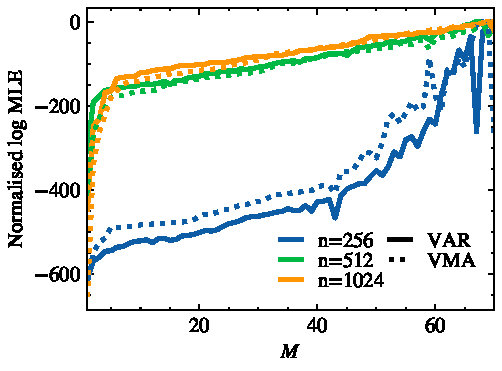
\includegraphics[width=\columnwidth]{sim_basis.pdf}
  \caption{The relationship between the number of basis functions and the maximum likelihood estimate for both VAR(2) and VMA1(1) models with different lengths. \avi{remake plot using $L_2$ instead of $L2$. Also speciofy the difference between a) and b) }}
  \label{sim_basis}
\end{figure}


\begin{figure}
  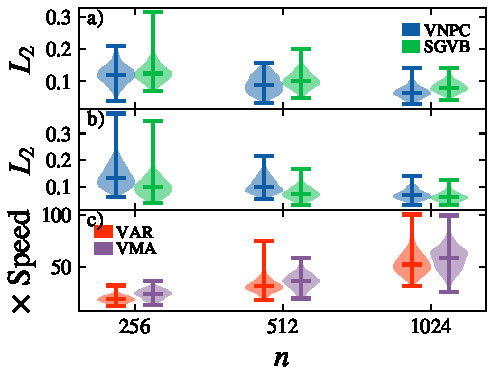
\includegraphics[width=\columnwidth]{sim_error_violins.pdf}
  \caption{
  Violin plots of 500  $L_2$ errors obtained from applying the VNPC and SGVB methods to 500 realizations of both VAR(2) and VMA(1) models with different sample sizes ($n = 256, 512, 1024$). The blue boxes represent the errors computed by the VNPC method, while the green boxes represent those obtained using the SGVB method.}
  \label{sim_error_violins}
\end{figure}



\subsection{Accuracy of binned Likelihood}

\begin{figure}[h]
  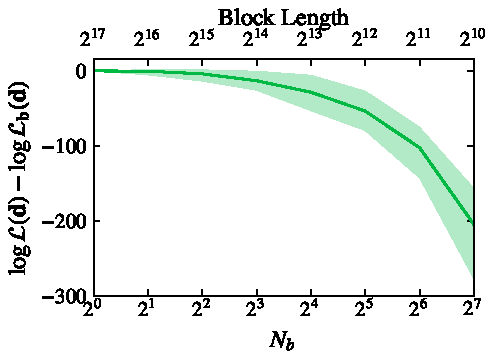
\includegraphics[width=\columnwidth]{lnl_vs_nchunks}
  \caption{Accuracy of the blocked  Whittle likelihood}
  \label{lnl_vs_nchunks}
\end{figure}




\section{Application to ET noise}
\label{sec:application}
\subsection{Data Generation}
We use 2000 seconds of  
%\avi{What is the sampling rate of the data?}
Gaussian noise colored with the design sensitivity of the
xylophone configuration of the ET sampled at 2048 Hz which yields a time series of length 4,096,000. \KJ{For some reason my footnote is not showing and I cannot figure out why. Look into fixing.}\RM{revtex puts them into the bibliography} \footnote{Please note that the sensitivity curve used here is the previously called `ET-D' sensitivity curve. We choose tho use this curve rather than the slightly updated version presented in \cite{Branchesi:2023mws}, to compare more directly to previous work \cite{Janssens2023}. The small difference between PSD curves will have no impact on the key conclusions of the applicability of the work presented in this paper.}~\cite{Hild_2009,Hild:2010id}. In the rest of the
paper we refer to this colored Gaussian noise as `ET noise' %\RM{What is the psd formula?} %\KJ{There is no straightforward formula. It is a complex combination from a handful key and another dozen smaller noise sources.}
% Note that despite the fact that
%we use identical noise, the X, Y and Z data are di
erent
%Gaussian noise realisations.
To simulate  non-identical correlated noise in the X, Y and Z channels, following \cite{Janssens2023}, we additionally injected another set of colored Gaussian noise, now with the shape of Gaussian peaks in the frequency domain. The Gaussian peaks are defined by the PSD
\[ S_n^{\mathrm{GP}}(f)= \left( \frac{A}{\sqrt{2\pi}}\exp\left\{ 
- \frac{(f-\mu)^2}{2\sigma^2}\right\}\right)^2\]
with amplitude $A$, frequency peak location $\mu$ and spread $\sigma$.
Gaussian noise was
injected in the X channel at $10$ Hz and 50 Hz, at 10
Hz and 90 Hz in the Y channel and at 50 Hz and 90 Hz in the Z channel with respective amplitudes at 10, 50 and 90 Hz of $4\times 10^{-24}$, $2\times 10^{-24}$ and $1.5\times 10^{-24}$ and $\sigma=1$ for all frequencies. Identical data was used for the Gaussian peaks at the same frequencies as to induce correlated noise between each pair of channels.
Whereas we recognize this dataset to be unrealistic in its simplicity and high level of separability due to the highly unique nature of the correlated noise terms (i.e. the Gaussian peaks), we believe it to be a good data set for initial demonstrations. Afterwards the goal is to increase complexity and approach a more realistic noise scenario such as the inclusion of correlated magnetic and/or Newtonian noise.



\subsection{Data Analysis}
\noindent
Case 1: correlated data - coherence \\
Case 2: uncorrelated data - coherence \\
Case 3: uncorrelated data - coherence = 0

\begin{itemize}
  \item Analysis of ET noise with coherently injected Gaussian peaks.
  \item Analysis of ET noise with incoherently injected Gaussian peaks.
  \begin{itemize}
      \item with the original SGVB method estimating the co-spectra
      \item with the modified SGVB method (off-diagonals not estimated) 
  \end{itemize}
\end{itemize}

In order to optimize the number of basis functions in the SGVB method for three cases, the effect of the number of basis functions on the maximum log Whittle likelihood is observed. The following plot illustrates the relationship between the number of basis functions and the corresponding maximized log Whittle likelihood values. During the maximization process, the learning rate for gradient ascent is set to 0.002, and the number of iterations is set to 10,000, with the number of basis functions ranging from 100 to 700 in increments of 10
\begin{figure}
\centering
  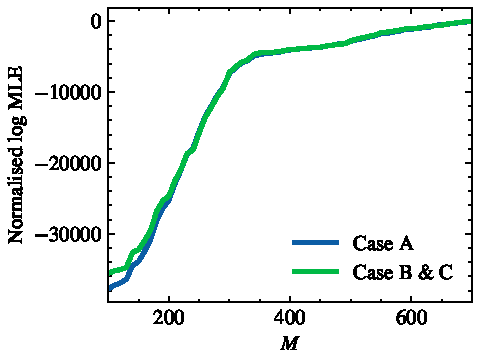
\includegraphics[width=\columnwidth]{et_basis_fns.pdf}
  \caption{The relationship between the number of basis functions and the maximum likelihood estimate for three cases. \avi{Set xlim to be the first and last M}}
  \label{et_corr_basis_funs_vs_mle}
\end{figure}

Based on the Figure ~\ref {et_corr_basis_funs_vs_mle}, the optimal number of basis functions for three cases can be set to 450. Python function Hyperopt is used to optimise the learning rate $\tau_1$ to maximise the ELBO, the range is set from 0.002 to 0.02 and the maximum number of evaluations is set to 10. The following plots (Figures \ref{fig:test} and \ref{caseAB_coh}) show the estimated power spectral densities and the squared coherences for three cases given the optimised learning rate and the corresponding parameters under the maximised ELBO.
\begin{figure*}[h]
\centering
\begin{subfigure}{\columnwidth}
  \centering
  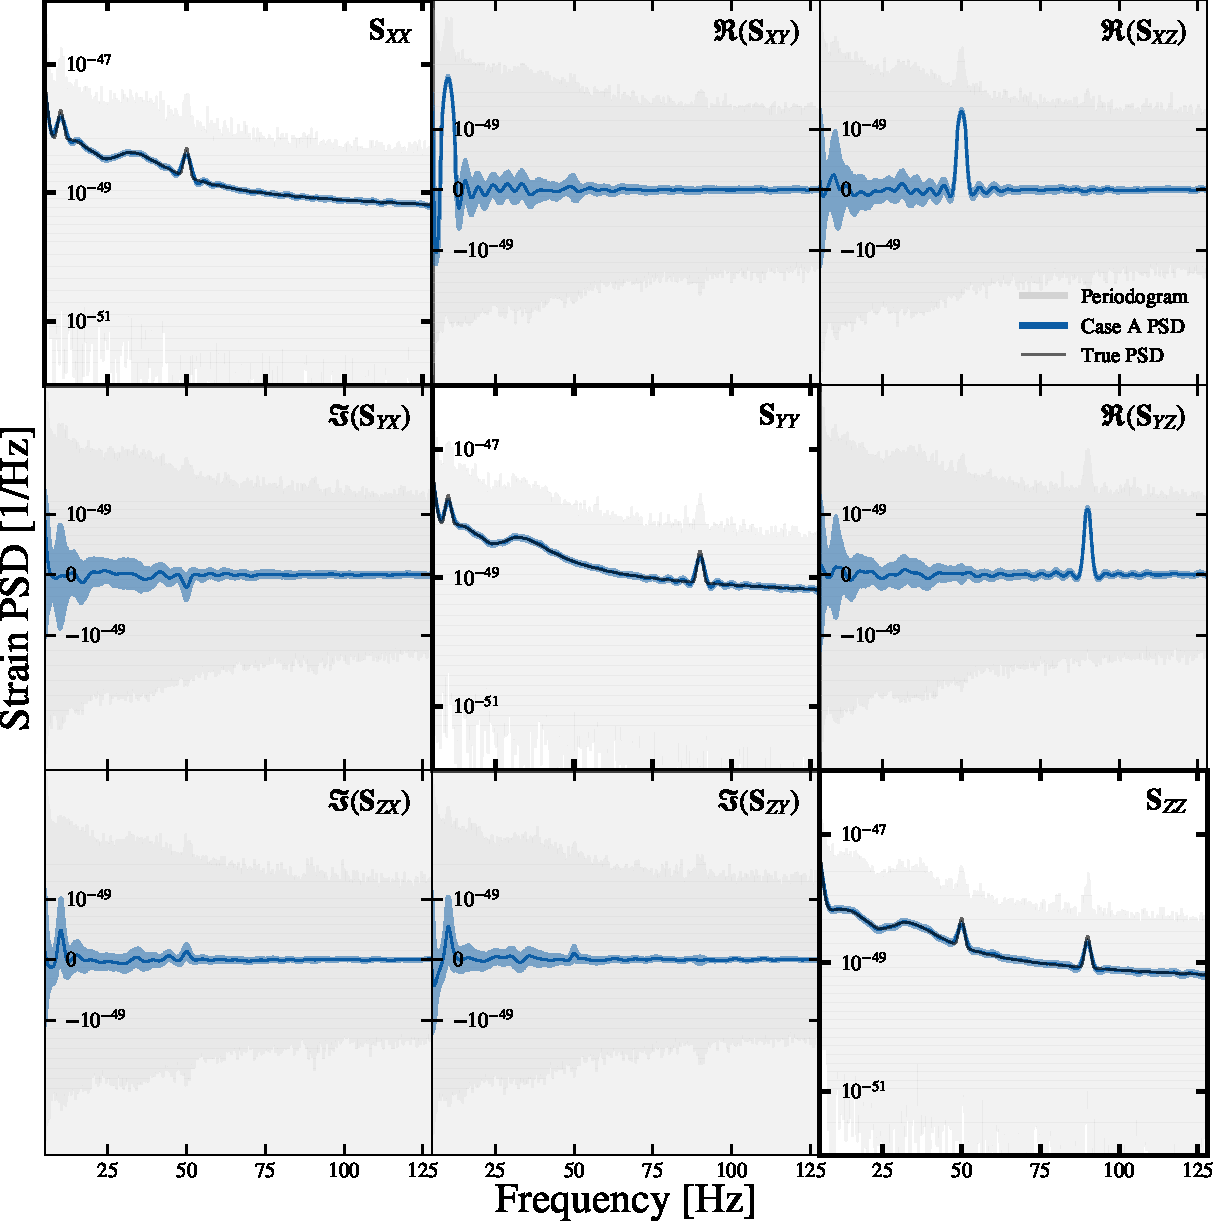
\includegraphics[width=1.05\columnwidth]{caseA_psd.pdf}
  \caption{Case A PSD}
  \label{fig:caseA_psd}
\end{subfigure}
\hfill
\begin{subfigure}{\columnwidth}
  \centering
  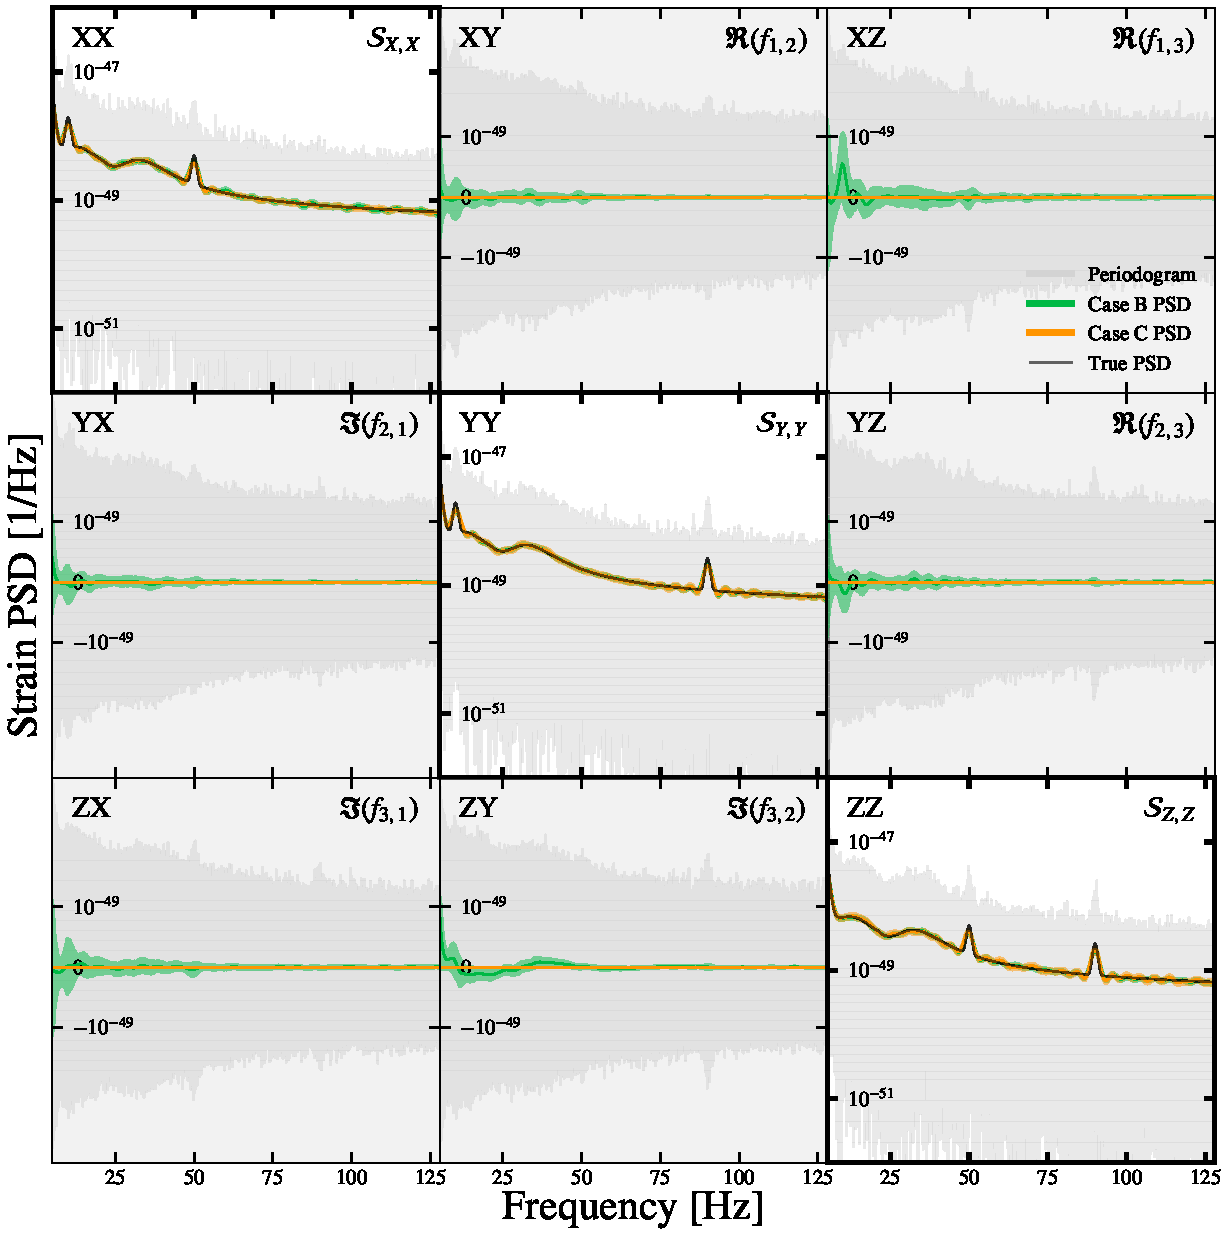
\includegraphics[width=1.05\columnwidth]{caseBC_psd.pdf}
  \caption{Case B and C PSD}
  \label{fig:caseBC_psd}
\end{subfigure}
\caption{Spectral density estimates for three cases of ET noise data. Estimates are shown for VI (SGVB, green with 90\% CI) and periodogram (grey).}
\label{fig:test}
\end{figure*}

\begin{figure}
  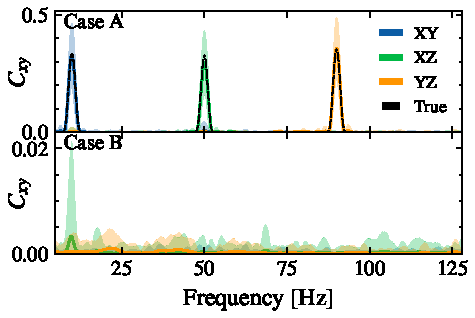
\includegraphics[width=\columnwidth]{caseAB_coh.pdf}
  \caption{Squared coherence estimates for differenct cases of ET noise data.}
  \label{caseAB_coh}
\end{figure}









\subsection{Results}
Show ET results, compare MCMC and SGVB on simulated ET noise with injected Gaussian peaks

\avi{Even if we can run the MCMC, comment on how long MCMC might take (estimate based on time for one LNL evaluation)}

\begin{itemize}
    \item VI Results, data with no correlation 
    \item VI Results, data with correlation
    \item VI no-off diagnals, data with correlation 
\end{itemize}



In this study, the SGVB method is utilized to estimate the spectral densities for the simulated data
of three channels, and construct the coherences for every pair of channels to obtain the correlation
between them in the certain frequencies. The dataset can be considered as a three dimensional
Gaussian stationary multivariate time series of length 4,096,000.
To handle such a large data set, in this study, the whole dataset is evenly divided into 125 
segments each of length 32,738, The Fourier-transformed
version of each segment serves as input data for a blocked Whittle likelihood. Every Whittle likelihood block with
corresponding input segment has the same basis function expressions for spectral density matrix.
Since the Fourier transform is an even function, the number of frequency points for each segment is
now 16384. Consequently, the product of 125 Whittle likelihood blocks forms
a new Whittle likelihood representing  the entire dataset. 
In this case, the hyperparameter $b$ in the regularized horseshoe prior is modified to $b = M$ , where
$M$ is the number of basis functions. This choice allows the model to utilize a larger number of basis
functions (up to 700). The increased flexibility enables the model to capture more complex patterns
in the data. The step sizes are set to be 0.005 and 0.05, respectively for each phase.

\section{Discussion}
\begin{itemize}
    \item demonstrated nonparametric methods to estimate correlated noise in ET (or LISA) data that can handle long time series 
    \item in future: simultaneous estimation of SGWB and noise
    \item hyperparameter optimization, adaptive learning rates
\end{itemize}


During the \ac{ET} era, managing correlated noise will be essential for maximising \ac{ET} scientific capabilities~\cite{Cireddu:2023:arXiv}.
We demonstrate a VI method for estimating a multivariate PSD for a \ac{GW} interferometer network under the influence of correlated noise and demonstrate how to quantify coherence. 
We demonstrate how the coherence changes as the noise correlation is adjusted. 
Future efforts will evaluate the impact of \ac{PE} for a compact-binary coalescence \ac{GW} signal in correlated noise, using a multivariate PSD and independent PSDs. 
Additional work will explore the automation of hyper-parameter optimisation to tune the \ac{VI} parameters. 


\begin{acknowledgments}
We like to thank Zhixiong Hu and Racquel Prado for making their code publicly available and for helpful discussions. NC, JEL, PMR, RM, and AV gratefully acknowledge support  by the Marsden Fund Council grant MFP-UOA2131 from New Zealand Government funding, managed by the Royal Society Te Apārangi. We thank the New Zealand eScience Infrastructure
(NeSI) \url{https://www.nesi.org.nz} for the use of their high performance computing facilities and
the Centre for eResearch at the University of Auckland for their technical
support.
\end{acknowledgments}
\bibliography{reference}

\appendix  

\section{Simulation study details}
\label{appdx:simstudy}
The VAR(2) model is defined by
\begin{align}
Z_t = \begin{pmatrix}0.5 & 0 \\0 & -0.3\end{pmatrix}\underline{Z}_{t-1}+\begin{pmatrix}0 & 0 \\0 & -0.5\end{pmatrix}\underline{Z}_{t-2}+\underline{e}_t, %\quad \underline{e}_t\overset{iid}{\sim}N \left(\bm{0}, \begin{pmatrix}1 & 0.9 \\0.9 & 1\end{pmatrix} \right)
\end{align}
 where $\underline{e}_t\overset{iid}{\sim}N \left(\bm{0}, \begin{pmatrix}1 & 0.9 \\0.9 & 1 \end{pmatrix}  \right) $ and the VMA(1) is given by
\begin{align}
\underline{Z}_t =\underline{e}_t+\begin{pmatrix}-0.75 & 0.5 \\0.5 & 0.75\end{pmatrix}\underline{e}_{t-1}, \quad \underline{e}_t\overset{iid}{\sim}N \left(\bm{0}, \begin{pmatrix}1 & 0.5 \\0.5 & 1\end{pmatrix}\right)\ .
\end{align}


Let $\hat{\bm{f}}$ denotes the estimated spectral density matrix for one realization, and let $\bm{f}_0$ be the true spectral density matrix. 
The $L_2$ error is defined as
\begin{eqnarray*}
||\hat{\bm{f}} - \bm{f}_0||_{L_2} &=& \left(\int_{0}^{0.5} ||\hat{\bm{f}}_0(\nu) - \bm{f}_0||^2 d\nu \right)^{\frac{1}{2}} \\
&\approx &\left(\frac{1}{N} \sum_{k=1}^{N}||\hat{\bm{f}}_0(\nu_k)-\bm{f}_0(\nu_k)||^2 \right)^{\frac{1}{2}}
\end{eqnarray*}
where $\Vert \cdot \Vert$ denotes the Frobenius norm, i.e., defined for a complex $p\times p$ matrix $\A$ by
$\displaystyle \Vert \A\Vert= \sqrt{\sum_{i,j} |a_{ij}|^2}$.





\end{document}
%
% ****** End of file apssamp.tex ******
